\documentclass[a4paper, 12pt, oneside, dvipsnames, table]{article}
\usepackage{../../../Utilita/Stiletemplate}
\usepackage{hyperref}
\usepackage{fancyhdr}
\usepackage[italian]{babel}
\usepackage[utf8]{inputenc}
\usepackage{float}
\usepackage{siunitx}
\usepackage{comment}
\usepackage{capt-of}
\restylefloat{table}

\newcommand{\Data}{2021\_01\_30}

\newcommand{\Titolo}{Verbale riunione \Data}

\newcommand{\Redattori}{\TL}

\newcommand{\Verificatori}{\PC}

\newcommand{\Approvatore}{\VD}

\newcommand{\Distribuzione}{\VT{} \newline \CR{} \newline Gruppo \Gruppo}

\newcommand{\Uso}{Interno}

\newcommand{\DescrizioneDoc}{Questo documento si occupa di riportare quanto discusso nella riunione del \Data.}

\newcommand{\pathimg}{../../../Immagini/N.O.S.jpg}

\newcommand{\Versionedoc}{1.0}
% info generali 
\newcommand{\NomeProgetto}{\textit{Emporio$\lambda$ambda}}

% fornitore
\newcommand{\Gruppo}{\textit{N.O.S}}
\newcommand{\Mail}{nos.unipd@gmail.com}

% committenti
\newcommand{\Committente}{\VT \newline \CR}
\newcommand{\VT}{Prof. Vardanega Tullio}
\newcommand{\CR}{Prof. Cardin Riccardo}

% proponenti
\newcommand{\Proponente}{\textit{RedBabel}}

% Componenti
\newcommand{\BL}{Brescanzin Lorenzo}
\newcommand{\FF}{Fantinato Filippo}
\newcommand{\MM}{Martini Matteo}
\newcommand{\PC}{Panighel Cristiano}
\newcommand{\TG}{Terrani Giulia}
\newcommand{\TL}{Tredese Leonardo}
\newcommand{\VD}{Varotto Davide}

% ruoli

\newcommand{\Responsabile}{\textit {Responsabile di Progetto}}
\newcommand{\Amministratore}{\textit{Amministratore di Progetto}}

% documenti

\newcommand{\SdF}{Studio di Fattibilità}
\newcommand{\SdFv}[1]{\textit{Studio di Fattibilità {#1}}}
\newcommand{\PdQ}{Piano di Qualifica}
\newcommand{\PdQv}[1]{\textit{Piano di Qualifica {#1}}}
\newcommand{\PdP}{Piano di Progetto}
\newcommand{\PdPv}[1]{\textit{Piano di Progetto {#1}}}
\newcommand{\NdP}{Norme di Progetto}
\newcommand{\NdPv}[1]{\textit{Norme di Progetto {#1}}}
\newcommand{\AdR}{Analisi dei Requisiti}
\newcommand{\AdRv}[1]{\textit{Analisi dei Requisiti {#1}}}
\newcommand{\Glossario}{Glossario}
\newcommand{\Glossariov}[1]{\textit{Glossario {#1}}}

% comandi generali
\newcommand{\glo}[1]{#1\ap{G}}

\newcommand{\myparagraph}[1]{\paragraph{#1}\mbox{}\\}

\setcounter{tocdepth}{5}  \setcounter{secnumdepth}{5}

	
\begin{document}

\copertina{}
\newpage

\fancydoc
\registroModifiche{
	
	2.0 & 2021\_03\_06 & \VD{} & Responsabile & - & Approvazione del documento. \\
	
	1.20 & 2021\_03\_05 & \MM{} & Analista & \TL{} & Inseriti UML corretti. \\
	
	1.19 & 2021\_03\_04 & \PC{} & Analista & \TL{} & Aggiornata sezione \S\ref{Tracciamento}. \\
	
	1.18 & 2021\_03\_02 & \PC{} & Analista & \BL{} & Aggiornata sezione \S\ref{ReqFunz}, requisiti del venditore. \\
	
	1.17 & 2021\_03\_01 & \MM{} & Analista & \PC{} & Aggiornata sezione \S\ref{ReqFunz}, requisiti dell'acquirente. \\
	
	1.16 & 2021\_02\_26 & \BL{} & Analista & \PC{} & Correzione dei precedenti e aggiunta di nuovi UC, estensioni di UC già presenti. \\

	1.15 & 2021\_02\_25 & \TG{} & Analista & \PC{} & Correzione UC "Lista riepilogo ordini" ora UC\ref{visualizzazione-ordini-in-gestione} e aggiunta UC da UC\ref{modifica-stato-ordine} a UC\ref{filtro-ordini-venditore}. \\
	
	1.14 & 2021\_02\_24 & \TG{} & Analista & \FF{} & Redatti nuovi UC\ref{ricerca-codice-ordine-acquirente} e UC\ref{filtro-temporale-ordini-acquirente}.\\
	
	1.13 & 2021\_02\_21 & \TG{} & Analista & \FF{} & Redatti nuovi UC\ref{inserimento-indirizzo-consegna}, UC\ref{modifica-indirizzo-consegna} e UC\ref{eliminazione-indirizzo-consegna}. \\
	
	1.12 & 2021\_02\_19 & \MM{} & Analista & \TG{} & Eliminato UC23-"Inserimento campo dati" e UC15-"Modifica informazioni profilo" ora suddiviso in UC\ref{modifica-informazioni-acquirente} e UC\ref{modifica-informazioni-venditore}. \\

	1.11 & 2021\_02\_18 & \PC{} & Analista & \BL{} & Correzione UC\ref{checkout}. \\

	1.10 & 2021\_02\_15 & \BL{} & Analista & \PC{} & Correzioni \S\ref{ReqVincolo} e \S\ref{ReqQual}, da UC\ref{aggiunta-carrello-plp} a UC\ref{modifica-quantita-nel-carrello}.\\
	
	1.9 & 2021\_02\_14 & \BL{} & Analista & \TG & Sistemazione UC\ref{logout} e UC\ref{ricerca-prodotti-acquirente}. \\
	
	1.8 & 2021\_02\_13 & \TG{} & Analista & \MM{} & Aggiunto i casi d'uso UC\ref{aggiunta-categoria}, UC\ref{modifica-categoria}, UC\ref{eliminazione-categoria}. \\

	1.7 & 2021\_02\_10 & \PC{} & Analista & \MM{} & Corretto i caso d'uso UC\ref{aggiunta-prodotto-evidenza} e UC\ref{rimozione-prodotto-evidenza}. \\

	1.6 & 2021\_02\_09 & \TG{} & Analista & \TL{} & Corretto le sezioni UC\ref{aggiunta-prodotto} e UC\ref{modifica-prodotto}. \\
	
	1.5 & 2021\_02\_08 & \MM{} & Analista & \FF{} & Trasformato sottocasi d'uso indipendenti relativi al venditore in casi d'uso. \\
	
	1.4 & 2021\_02\_04 & \MM{} & Analista & \PC{} & Trasformato sottocasi d'uso indipendenti relativi all'acquirente in casi d'uso. \\

	1.3 & 2021\_02\_03 & \TG{} & Analista & \TG{} & Rimossi i dettagli implementativi dai casi d'uso. Eliminato UC3-"Accesso al menù". \\

	1.2 & 2021\_02\_02 & \PC{} & Analista & \TL{} & Separati i casi di accesso alla piattaforma sezione \S\ref{AccessoPiattaforma}. \\

	1.1 & 2021\_02\_02 & \BL{} & Analista & \FF{} & Rimosso l'attore amministratore sezione \S\ref{Attori}. \\ 

	1.0.0 & 2021\_01\_10 & \PC{} & Responsabile & - & Approvazione del documento. \\
	
	0.1.7 & 2021\_01\_09 & \FF{} & Analista & \TL{} & Stesura riepilogo tracciamento \S\ref{Riepilogo} \\
	
	0.1.6 & 2021\_01\_09 & \TL{} & Analista & \BL{} & Stesura tracciamento requisito-fonte \S\ref{ReqFonte} \\
	
	0.1.5 & 2021\_01\_09 & \BL{} & Analista & \FF{} & Stesura tracciamento fonte-requisito \S\ref{FonteReq} \\
	
	0.1.4 & 2021\_01\_08 & \MM{} & Analista & \BL{} & Aggiunta diagrammi dei casi d'uso \S\ref{CasiUso} \\
	
	0.1.3 & 2021\_01\_08 & \TL{} & Analista & \TG{} & Stesura requisiti vincolo \S\ref{ReqVincolo} e prestazionali \S\ref{ReqPrest} \\
	
	0.1.2 & 2021\_01\_08 & \FF{} & Analista & \TG{} & Stesura requisiti di qualità \S\ref{ReqQual} \\
	
	0.1.1 & 2021\_01\_07 & \BL{} & Analista & \TG{} & Stesura requisiti funzionali \S\ref{ReqFunz} \\
	
	0.1.0 & 2021\_01\_06 & - & - & \TG{} & Verifica complessiva del documento. \\
	
	0.0.10  & 2020\_12\_27 & \FF{} & Analista & \TG{} & Stesura caso d'uso UC\ref{estensione:limite-foto-raggiunto}, UC\ref{estensione:prezzo-minore-o-uguale-zero}, UC\ref{estensione:email-non-esistente}, UC\ref{estensione:registrazione-con-email-non-esistente}, UC\ref{estensione:quantita-da-aggiungere-al-carrello-non-valida}, UC\ref{estensione:sconto-minore-zero}, UC\ref{estensione:pagamento-fallito}, UC\ref{estensione:sconto-maggiore-cento} \\
	
	0.0.9 & 2021\_01\_05 & \BL{} & Analista & \TG{} & Stesura casi d'uso: UC\ref{estensione:cambio-con-email-esistente}, UC\ref{estensione:campo-obbligatorio-non-inserito}, UC\ref{estensione:credenziali-non-presenti}, UC\ref{estensione:email-non-valida}, UC\ref{estensione:file-no-tipo-immagine} \\
	
	0.0.8 & 2021\_01\_04 & \TL{} & Analista & \TG{} & Aggiornamento sezioni UC\ref{eliminazione-prodotto}, UC\ref{aggiunta-prodotto-evidenza}, UC\ref{rimozione-prodotto-evidenza}, UC\ref{rifornimento-prodotto} \\
	
	0.0.7 & 2021\_01\_04 & \TL{} & Analista & \TG{} & Aggiornamento sezioni UC\ref{modifica-informazioni-venditore}, UC\ref{eliminazione-account-acquirente}, UC\ref{aggiunta-prodotto}, UC\ref{modifica-prodotto} e \S\ref{Attori} \\
	
	0.0.6 & 2021\_01\_03 & \BL{} & Analista & \TG{} & Stesura casi d'uso: UC\ref{modifica-quantita-da-aggiungere-al-carrello}, UC\ref{eliminazione-prodotto-dal-carrello}, UC\ref{checkout}, UC\ref{visualizzazione-ordini-effettuati}, UC\ref{modifica-informazioni-acquirente} \\
	
	0.0.5  & 2021\_01\_02 & \BL{} & Analista & \TG{} & Stesura casi d'uso: UC\ref{ordinamento-prezzo-decrescente}, UC\ref{aggiunta-carrello-pdp}, UC\ref{aggiunta-carrello-plp} \\
	
	0.0.4  & 2021\_01\_02 & \FF{} & Analista & \TG{} & Stesura casi d'uso: UC\ref{logout}, UC\ref{ricerca-prodotti-acquirente}, UC\ref{filtro-prodotti-acquirente}, UC\ref{ordinamento-prezzo-crescente} \\
	
	0.0.3  & 2021\_01\_01 & \FF{} & Analista & \TG{} & Stesura casi d'uso: UC\ref{registrazione}, UC\ref{autenticazione-acquirente}, UC\ref{autenticazione-venditore}, UC\ref{password-dimenticata} \\ 
	
	0.0.2  & 2020\_12\_27 & \TG{} & Analista & \TL{} & Stesura \S\ref{Desc} \\  
	
	0.0.1  & 2020\_12\_22 & \TG{} & Analista & \BL{} & Stesura scheletro del documento, \S\ref{Intro}, \S\ref{Desc} \\
}

\setcounter{table}{0}

\clearpage
\tableofcontents
\clearpage

\listoffigures
\newpage

\section{Introduzione}
\subsection{Scopo del Documento}
Questo documento contiene la stesura dello studio di fattibilità riguardante i sette capitolati proposti, elencando quelli che il nostro gruppo ha considerato come i loro aspetti più interessanti e le loro criticità. Infine, per ogni capitolato vengono esposte le motivazioni e le ragioni per cui il gruppo ha scelto come progetto il capitolato C2 \NomeProgetto{} a discapito degli altri sei proposti.

\subsection{Glossario}
Al fine di evitare ambiguità fra i termini, e per avere le terminologie chiare fra tutti gli stakeholder, il gruppo \Gruppo{} ha redatto un documento denominato \Glossariov{1.0.0}.
In tale documento sono presenti tutti i termini tecnici, ambigui, specifici del progetto e scelti dai membri del gruppo con le loro relative definizioni.
Un termine presente nel \Glossariov{1.0.0} e utilizzato in questo documento viene indicato con un apice \ap{G} alla fine della parola.

\subsection{Riferimenti}

\subsubsection{Normativi}
\begin{itemize}
\item \NdPv{1.0.0}.
\end{itemize}

\subsubsection{Informativi}

\begin{itemize}
\item \textbf {Capitolato d'appalto C1 - BlockCOVID:}\\
\url{https://www.math.unipd.it/~tullio/IS-1/2020/Progetto/C1.pdf}
\item \textbf {Capitolato d'appalto C2 - \NomeProgetto:}\\
\url{https://www.math.unipd.it/~tullio/IS-1/2020/Progetto/C2.pdf}
\item \textbf {Capitolato d'appalto C3 - Gathering Detection Platform:}\\
\url{https://www.math.unipd.it/~tullio/IS-1/2020/Progetto/C3.pdf}
\item \textbf {Capitolato d'appalto C4 - HD Viz:}\\
\url{https://www.math.unipd.it/~tullio/IS-1/2020/Progetto/C4.pdf}
\item \textbf {Capitolato d'appalto C5 - PORTACS:}\\
\url{https://www.math.unipd.it/~tullio/IS-1/2020/Progetto/C5.pdf}
\item \textbf {Capitolato d'appalto C6 - Realtime Gaming Platform:}\\
\url{https://www.math.unipd.it/~tullio/IS-1/2020/Progetto/C6.pdf}
\item \textbf {Capitolato d'appalto C7 - SSD:}\\
\url{https://www.math.unipd.it/~tullio/IS-1/2020/Progetto/C7.pdf}

\end{itemize}
\newpage

\section{Tecnologie, framework e librerie impiegate}
Di seguito vengono descritte tecnologie, framework e servizi di terze parti utilizzati per il progetto.
\subsection{Swagger}
Swagger è un linguaggio di descrizione dell'interfaccia per descrivere le API RESTful espresse utilizzando JSON. Swagger viene utilizzato insieme a una serie di strumenti software open source per progettare, creare, documentare e utilizzare i servizi Web RESTful.
\subsection{AWS Cognito}
AWS Cognito fornisce autenticazione, autorizzazione e gestione degli utenti per le applicazioni Web e mobili. Gli utenti possono accedere direttamente con un nome utente e una password, oppure tramite terze parti, ad esempio Facebook, Amazon, Google o Apple.
I due componenti principali di Amazon Cognito da utilizzare separatamente o insieme sono i pool di utenti, directory utente che forniscono opzioni di registrazione e di accesso, e i pool di identità che consentono di concedere agli utenti l'accesso ad altri servizi AWS.
\subsection{AWS DynamoDB} 
Amazon DynamoDB è un database NoSQL che offre prestazioni veloci e predicibili, in particolare si tratta di un database completamente gestito che consente di scaricare gli oneri amministrativi legati al funzionamento e al ridimensionamento di un database distribuito in modo da non doversi preoccupare del provisioning, dell'installazione e della configurazione dell'hardware, della replica, delle patch del software o del ridimensionamento del cluster eliminando il carico operativo e la complessità coinvolti nella protezione dei dati sensibili. 

\subsection{AWS API Gateway}
Amazon API Gateway semplifica per gli sviluppatori la creazione, la pubblicazione, la manutenzione, il monitoraggio e la protezione delle API RESTful su qualsiasi scala. Le API fungono da “porta di entrata” per consentire l’accesso delle applicazioni ai dati, alla logica aziendale o alle funzionalità dai servizi back-end. 
API Gateway gestisce tutte le attività di accettazione ed elaborazione relative a centinaia di migliaia di chiamate API simultanee, inclusi gestione del traffico, controllo di accessi e autorizzazioni, monitoraggio e gestione delle versioni delle API. 

\subsection{AWS Lambda}
AWS Lambda è un servizio di elaborazione serverless che permette di eseguire il codice senza effettuare il provisioning o gestire i server, creare una logica di dimensionamento dei cluster in funzione dei carichi di lavoro, mantenere integrazioni degli eventi o gestire i runtime. Con Lambda è possibile eseguire codice per qualsiasi tipo di applicazione o servizio di back-end, senza alcuna amministrazione.  È possibile scrivere le funzioni Lambda nel linguaggio preferiro (Node.js, Python, Go, Java e altri ancora) e utilizzare strumenti sia serverless sia di container, come AWS SAM o Docker CLI, per creare, testare e distribuire le funzioni.
\subsection{Amazon S3 Bucket}
È un servizio di storage di oggetti che offre scalabilità, disponibilità dei dati, sicurezza e prestazioni all'avanguardia nel settore offrendo caratteristiche di gestione semplici da utilizzare che consentono di organizzare i dati e di configurare controlli di accesso ottimizzati per soddisfare requisiti aziendali, di pianificazione e di conformità specifici.
\subsection{Amazon SNS}
Amazon Simple Notification Service (Amazon SNS) è un servizio di messaggistica completamente gestito per la comunicazione application-to-person (A2P) e application-to-application (A2A).
Le comunicazioni avvengono in modo asincrono, con un punto di accesso logico e un canale di comunicazione. 
\subsection{Amazon SQS}
Amazon Simple Queue Service (SQS) è un servizio di accodamento messaggi completamente gestito che consente la separazione e la scalabilità di microservizi, sistemi distribuiti e applicazioni serverless. Con SQS, è possibile inviare, memorizzare e ricevere qualsiasi volume di messaggi tra componenti software senza perdite e senza dover impiegare altri servizi per mantenere la disponibilità. 
SQS offre due tipi di code di messaggi: le code standard offrono throughput massimo, ordinamento semplificato e distribuzione di tipo at-least-once mentre le code FIFO sono progettate per garantire che i messaggi vengano elaborati esattamente una sola volta, nell'ordine in cui sono inviati.
\subsection{Stripe}
Stripe è una piattaforma esterna per i pagamenti online che consente all'e-commerce di accettare pagamenti con bancomat, carta ricaricabile o carta di credito. È una soluzione sicura e rapida, i pagamenti vengono elaborati utilizzando strumenti ad hoc sviluppati per la gestione dei flussi di pagamento con controlli anti-frode.
\subsection{NodeJs}
Node.js è un runtime system open source multipiattaforma orientato agli eventi per l'esecuzione di codice JavaScript, ha un'architettura orientata agli eventi che rende possibile l’I/O asincrono. Questo design punta ad ottimizzare il Throughput e la scalabilità nelle applicazioni web con molte operazioni di input/output. Il modello di networking su cui si basa Node.js è I/O event-driven: ciò vuol dire che Node richiede al sistema operativo di ricevere notifiche al verificarsi di determinati eventi, e rimane quindi in sleep fino alla notifica stessa: solo in tale momento torna attivo per eseguire le istruzioni previste nella funzione di callback, così chiamata perché da eseguire una volta ricevuta la notifica che il risultato dell'elaborazione del sistema operativo è disponibile.
\subsection{Npm}
Npm è un package manager per il linguaggio di programmazione JavaScript, il predefinito per l'ambiente di runtime JavaScript Node.js. Consiste in un client da linea di comando, chiamato anch'esso npm, e un database online di moduli pubblici e privati che offrono diverse funzionalità: dalla gestione dell’upload di file, ai database MySQL o a Redis, attraverso framework, sistemi di template e la gestione della comunicazione in tempo reale con i visitatori.
\subsection{TypeScript}
TypeScript è un linguaggio di programmazione open source sviluppato da Microsoft che estende la sintassi di JavaScript, aggiungendo o rendendo più flessibili e potenti varie sue caratteristiche, in modo che qualunque programma scritto in JavaScript sia anche in grado di funzionare con TypeScript senza nessuna modifica. 
\subsection{Next.js}
Next.js è un framework JavaScript back-end per applicazioni React che non richiede alcun setup e che consente il rendering automatico lato server (SSR, server side rendering).
Con Next.js si possono sviluppare applicazioni web, app mobile, desktop e web app progressive: è costruito secondo il principio di “Build once, run anywhere“.
Altre caratteristiche di Next.js sono suddivisione automatica del codice, routing automatico, hot code reloading (viene ricaricato solo il codice modificato) ed esportazione statica (con un solo comando può esportare un sito statico).
\subsection{Jest.js}
Jest.js è un framework di test JavaScript con particolare attenzione alla semplicità e al supporto per applicazioni web di grandi dimensioni.  Fornisce diverse funzionalità come la creazione automatizzata di mock, l'esecuzione di test in parallelo per aumentarne la velocità e la possibilità di testare il codice asincrono in modo sincrono. Jest trova automaticamente i test da eseguire nel codice sorgente, e funziona su progetti JS che includono React, Babel, TypeScript, Node, Angular, Vue.
\subsection{ESLint}
ESLint è uno strumento di analisi del codice statico per identificare pattern problematici o codice che non rispetta certe linee guida predefinite nel codice JavaScript senza eseguirlo. Le regole in ESLint sono configurabili e le regole personalizzate possono essere definite e caricate. ESLint è scritto usando Node.js per fornire un ambiente a runtime veloce e di facile installazione attraverso npm.
\subsection{Material-UI}
Material-UI è una libreria di componenti React per sviluppare il design del proprio progetto o per poter utilizzare tutta una serie di componenti stabili predefiniti.
\subsection{Serverless Framework}
Serverless Framework è un framework Web gratuito e open source scritto utilizzando Node.js, sviluppato per la creazione di applicazioni su AWS Lambda. Il Serverless Framework è costituito da una CLI open source e da una dashboard che insieme, forniscono una gestione completa del ciclo di vita delle applicazioni serverless.

\section{Setup della piattaforma}\label{Setup}
\subsection{Requisiti minimi}
Per il deploy della piattaforma \NomeProgetto\ è necessario disporre di un account AWS valido per ottenere le credenziali da includere nella configurazione del profilo del framework serverless.
Il sistema dove verrà effettuato il deploy deve avere installato:
\begin{itemize}
	\item Npm;
	\item NodeJS;
	\item Serverless framework.
\end{itemize}
Di seguito sono riportati i sistemi operativi e i browser che supportano la piattaforma.
\begin{itemize}
	\item \textbf{Sistemi operativi}:
	\item \textbf{Browser}:
\end{itemize}

\subsection{Deploy}
Per il deploy della piattaforma, seguire i seguenti passi:
\begin{itemize}
	\item Aprire una \glo{CLI} e posizionarsi nella cartella dove sono contenuti i file;
	\item Installare le dipendenze usando il comando \textbf{npm install};
	\item Creare una nuova applicazione serverless lanciando il comando \textbf{serverless};
	\item Iniziare il deploy della piattaforma \NomeProgetto\ lanciando il comando \textbf{serverless deploy}.
\end{itemize}

\subsection{Test}
L'analisi statica del codice redatto viene effettuata dal linter EsLint.\\
Per i test di unità è stato impiegato il framework Jest.js.
\section{Backend}
\subsection{Descrizione generale}\label{beDescrizione}
Le funzionalità previste dalla piattaforma hanno permesso di individuare i seguenti domini:
\begin{itemize}
	\item \textbf{Products;}
	\item \textbf{Categories;}
	\item \textbf{Payments;}
	\item \textbf{Orders;}
	\item \textbf{Cart;}
	\item \textbf{Addresses;}
	\item \textbf{Users.}
\end{itemize}
I domini sono stati uniti riflettendo sulle loro interdipendenze al fine di individuare dei \glo{microservizi} utili per procedere con lo sviluppo, in particolare sono stati identificati i microservizi:
\begin{itemize}
	\item \textbf{Products-categories service;}
	\item \textbf{Payments-orders service;}
	\item \textbf{Carts service;}
	\item \textbf{Addresses service;}
	\item \textbf{Users service.}
\end{itemize}
Lo sviluppo di singoli servizi permette una maggiore possibilità di sviluppo in parallelo dei singoli domini grazie alla loro struttura e all'agilità degli aggiornamenti e la possibilità di gestire i dati in modo decentralizzato.

\subsection{Struttura dei microservizi}\label{StrutturaMicroservizi}
\begin{figure}[H]
	\centering
	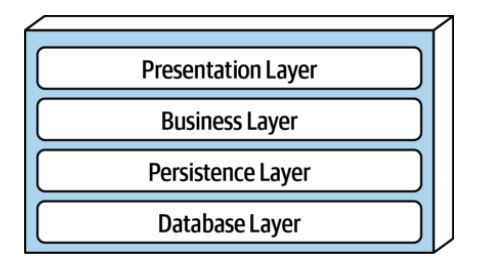
\includegraphics[scale=0.4]{Immagini/Backend/layer.png}
	\caption{layered architecture}
	\label{fig:layer}
\end{figure}
La struttura di ogni singolo servizio si basa su una \textbf{layered architecture} dove i componenti sono organizzati in vari strati che comunicano tra loro, il principale vantaggio è che risulta molto più semplice procedere ai test attraverso \glo{mock}.\\
Andando ad analizzare il singolo microservizio abbiamo:
\begin{center}
	\begin{minipage}{0.3\textwidth}
		\centering
		
\includegraphics[scale=0.78]{Immagini/Backend/Amazon-DynamoDB.png}
		\captionof{figure}{DynamoDB}
	\end{minipage}
	\begin{minipage}{0.3\textwidth}
		\centering
		
\includegraphics[scale=0.19]{Immagini/Backend/AWSLambda.png}
		\captionof{figure}{Lambda}
	\end{minipage}
	\begin{minipage}{0.3\textwidth}
		\centering
		
\includegraphics[scale=0.26]{Immagini/Backend/Gateway.png}
		\captionof{figure}{API Gateway}
	\end{minipage}
\end{center}
\begin{itemize}
	\item \textbf{DynamoDB:} per gestire i vari dati;
	\item \textbf{Lambda:} le funzioni che lavorano sui dati del database;
	\item \textbf{API Gateway:} riceve e gestisce le richieste del client richiamando le lambda e restituendone i risultati.
\end{itemize}

\subsubsection{Products-categories service}
\begin{figure}[H]
	\centering
	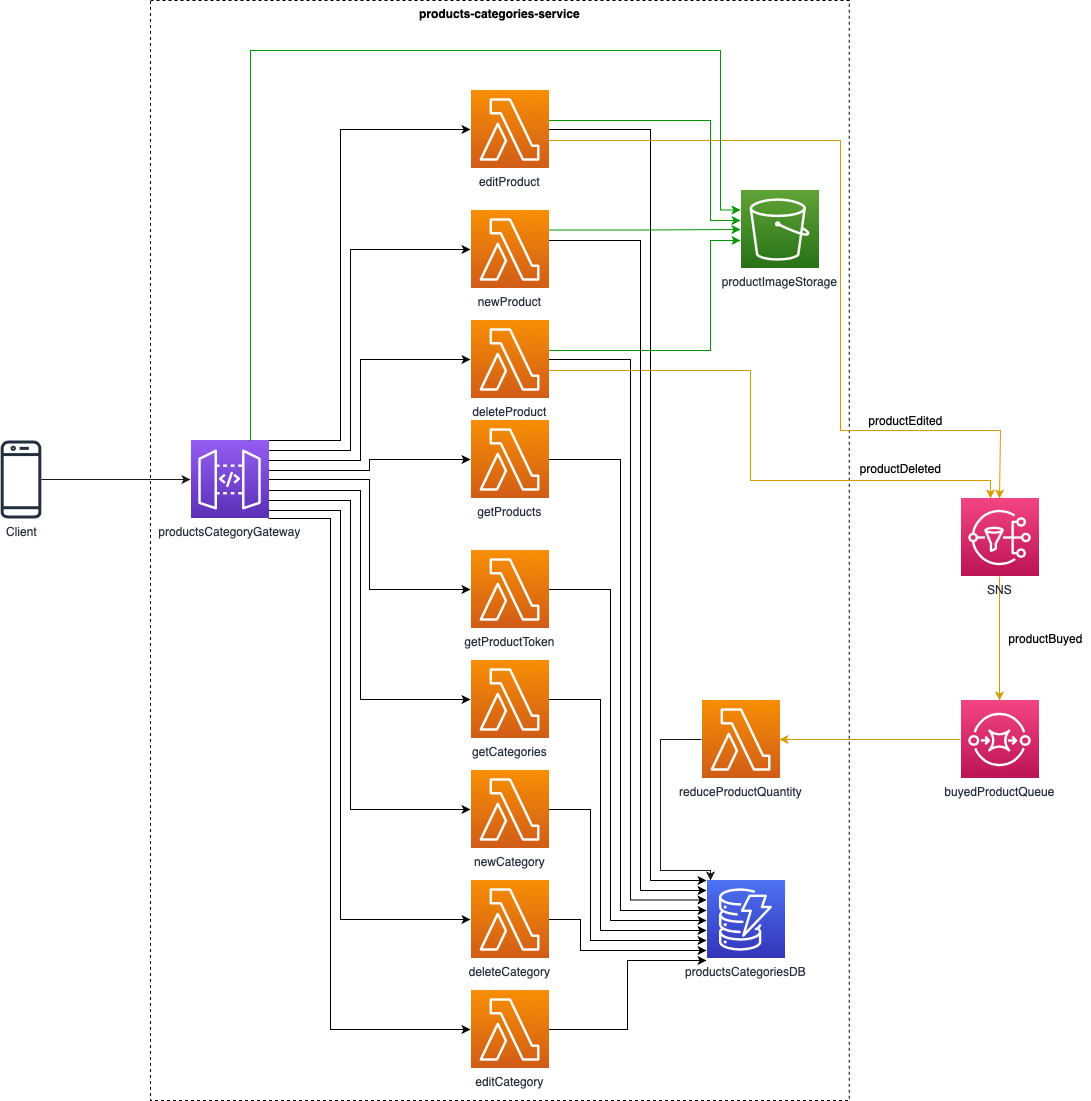
\includegraphics[scale=0.4]{Immagini/Backend/AWSProductsCategories.png}
	\caption{Products-categories service}
	\label{fig:ProductCategories}
\end{figure}
Il microservizio \textbf{products-categories} fornisce le principali funzionalità per gestire i prodotti e le categorie alle quali vengono assegnati per le funzioni di ricerca. Sono esempi di funzioni usufruibili dall'utente:
\begin{itemize}
	\item Inserimento di un nuovo prodotto;
	\item Eliminazione di un prodotto già presente nella piattaforma;
	\item Modifica delle specifiche di un prodotto;
	\item Inserimento di una nuova categoria per la classificazione dei vari prodotti in vendita.
\end{itemize}\noindent
Oltre all'utilizzo come per i successivi microservizi di AWS API Gateway, AWS Lambda e AWS DynamoDB viene impiegato Amazon S3 bucket per gestire le immagini associate ad un prodotto e Amazon SNS e SQS permettono il controllo della modifica/eliminazione di un prodotto assicurando la corretta validità della quantità disponibile dello stesso.

\subsubsection{Payments-orders service}
\begin{figure}[H]
	\centering
	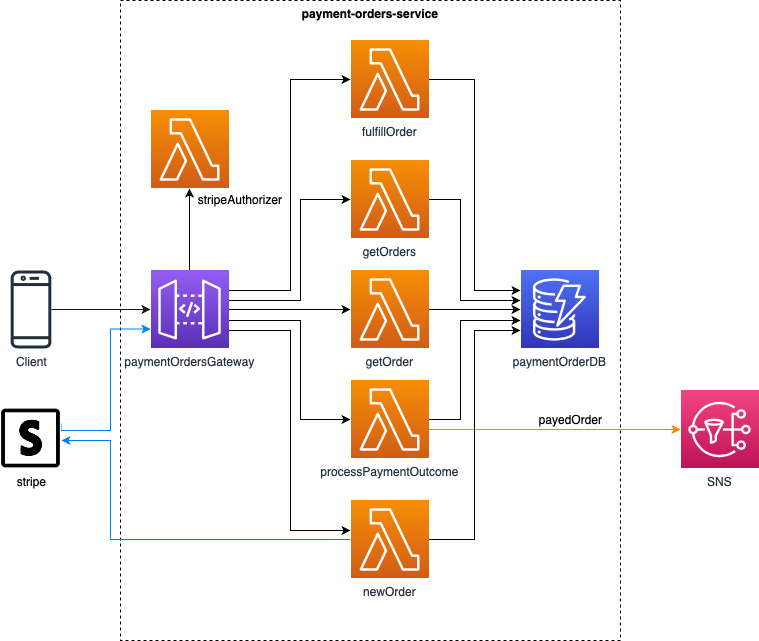
\includegraphics[scale=0.4]{Immagini/Backend/AWSPaymentOrders.png}
	\caption{Payments-orders service}
	\label{fig:Payment-orders}
\end{figure}
Il microservizio \textbf{payments-orders} fornisce le principali funzionalità per gestire il pagamento di un ordine e garantire la storicizzazione degli ordini effettuati. Anche in questo microservizio viene utilizzato Amazon SNS per assicurare il corretto risultato del pagamento, gestito dal servizio esterno Stripe.

\subsubsection{Carts service}
\begin{figure}[H]
	\centering
	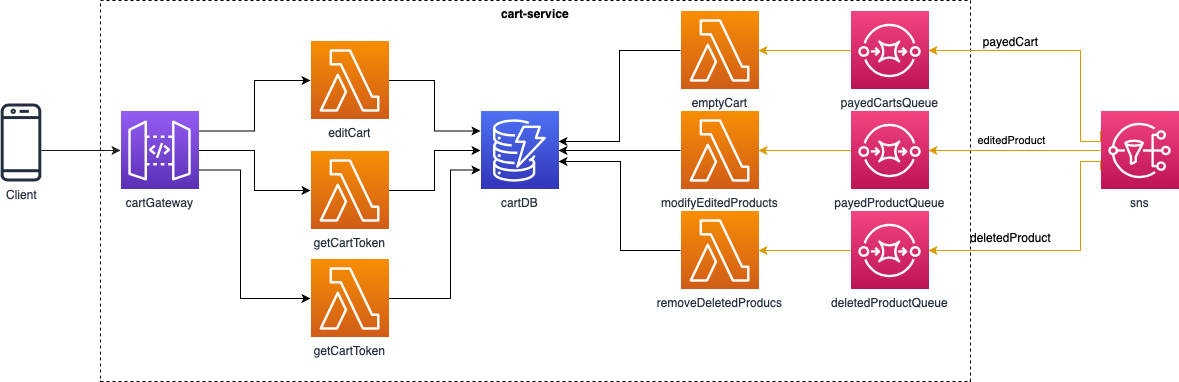
\includegraphics[scale=0.4]{Immagini/Backend/AWSCart.png}
	\caption{Carts service}
	\label{fig:Cart}
\end{figure}
Il microservizio \textbf{carts} fornisce le principali funzionalità per gestire il carrello dell'utente assicurando che eventuali modifiche fatte sui suoi prodotti esternamente, ad esempio il venditore modifica il prezzo di un prodotto, si riflettano anche all'interno dei carrelli degli utenti attraverso l'utilizzo di Amazon SNS e SQS.

\subsubsection{Addresses service}
\begin{figure}[H]
	\centering
	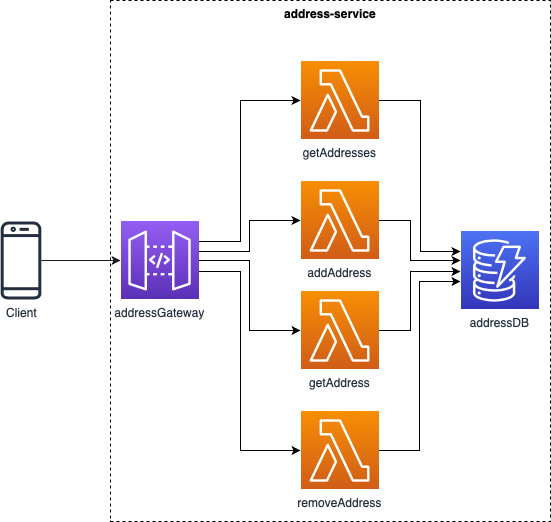
\includegraphics[scale=0.4]{Immagini/Backend/AWSAddresses.png}
	\caption{Addresses service}
	\label{fig:Adresses}
\end{figure}
Il microservizio \textbf{addresses} fornisce le principali funzionalità per gestire gli indirizzi di spedizione di un utente come l'aggiunta o la rimozione di un indirizzo. In questo microservizio entrano in gioco solo AWS API Gateway, AWS Lambda e AWS DynamoDB.

\subsubsection{Users service}
\begin{figure}[H]
	\centering
	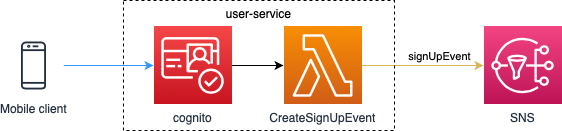
\includegraphics[scale=0.7]{Immagini/Backend/AWSUserService.png}
	\caption{Users service}
	\label{fig:Users}
\end{figure} 
Il microservizio \textbf{users} fornisce le principali funzionalità per gestire la registrazione e l'autenticazione di un utente alla piattaforma attraverso l'utilizzo di AWS Cognito.

\subsection{Struttura del backend}\label{Strutturabe}
\begin{figure}[H]
	\centering
	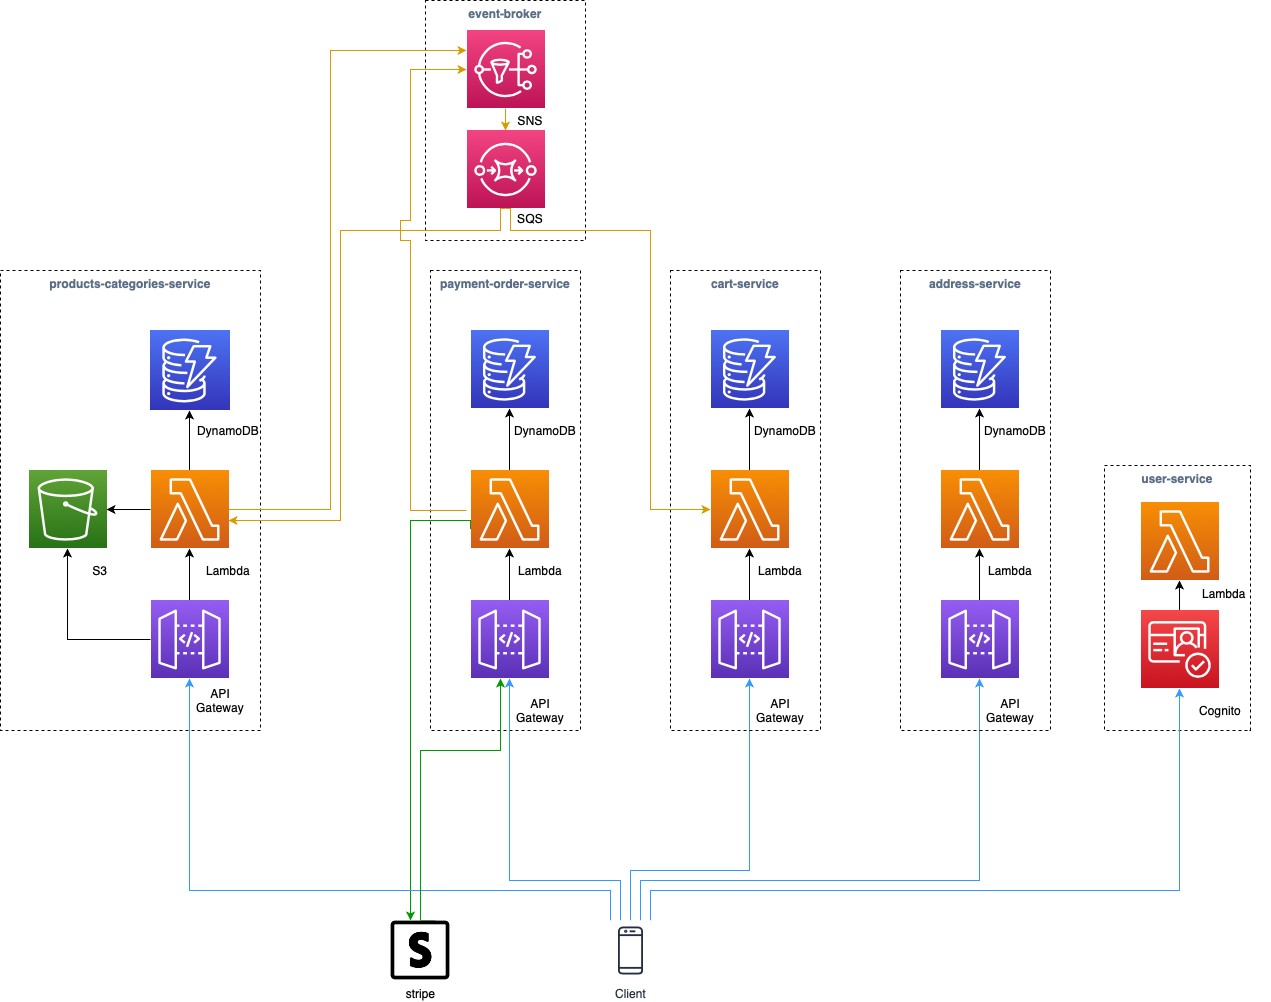
\includegraphics[scale=0.4]{Immagini/Backend/AWSArchitecture.png}
	\caption{Architettura backend}
	\label{fig:backend}
\end{figure}
Per slegare i microservizi tra di loro vengono utilizzate due strategie. La prima consiste nel gestire le chiamate asincrone attraverso SNS il servizio che fa da \glo{event broker} su AWS, eliminando così lo sviluppo di integrazioni tra microservizi e limitandosi a quelle per il \glo{message broker}.
La seconda invece è pensata per eliminare le chiamate sincrone tra microservizi, come quelle di validazione. Per far ciò si utilizza la firma digitale legata a un microservizio per verificare l'integrità delle richieste del client, sostituendo così le varie integrazioni necessarie a un semplice check attraverso la chiave pubblica del microservizio.

\subsection{Diagrammi di sequenza}\label{Diagrammiseq}
Di seguito sono riportati i diagrammi di sequenza per descrivere alcune delle principali operazioni effettuabili all'interno della piattaforma.
\subsubsection{Creazione ed eliminazione di un prodotto effettuata dal venditore}
\begin{figure}[H]
	\centering
	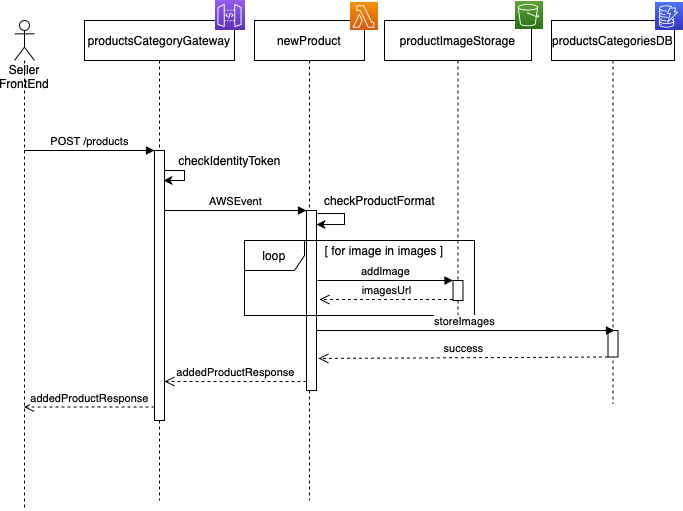
\includegraphics[scale=0.5]{Immagini/Backend/CreazioneProdotto.png}
	\caption{Creazione di un nuovo prodotto nella piattaforma}
	\label{fig:DiagrammaCreazioneProdotto}
\end{figure}
\begin{figure}[H]
	\centering
	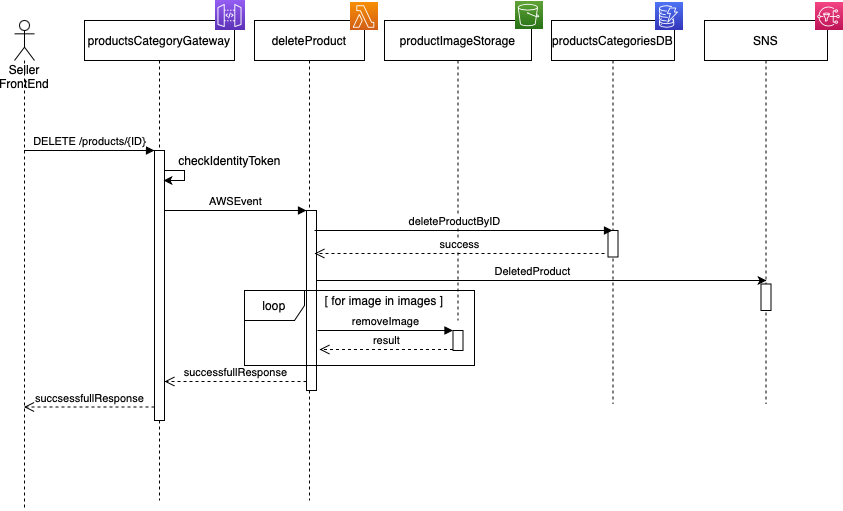
\includegraphics[scale=0.47]{Immagini/Backend/EliminazioneProdotto.png}
	\caption{Eliminazione di un prodotto dalla piattaforma}
	\label{fig:DiagrammiEliminazioneProdotto}
\end{figure}
I diagrammi rappresentano rispettivamente la creazione e l'eliminazione di un prodotto dalla piattaforma, in queste operazioni è necessario prevedere la gestione del salvataggio delle eventuali immagini associate ai prodotti tramite Amazon S3 bucket.
\subsubsection{Aggiunta di un prodotto al carrello}
\begin{figure}[H]
	\centering
	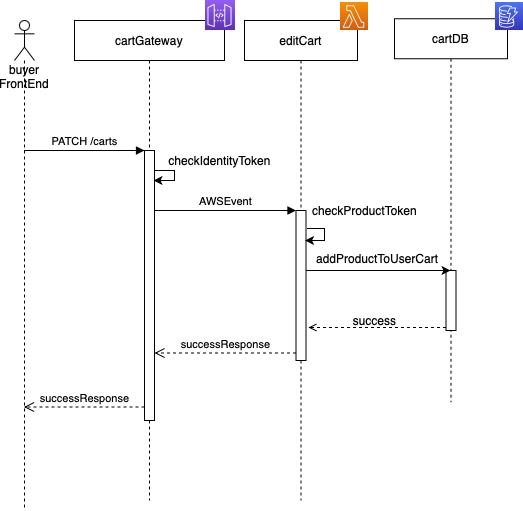
\includegraphics[scale=0.5]{Immagini/Backend/AggiuntaProdottoAlCarrello.png}
	\caption{Aggiunta di un prodotto al carrello}
	\label{fig:DiagrammaCarrello}
\end{figure}
Il diagramma rappresenta l'interazione delle tecnologie quando l'utente aggiunge un nuovo prodotto al carrello, in questo caso occorre modificare lo stato del carrello.
\subsubsection{Modifica di un indirizzo di spedizione}
\begin{figure}[H]
	\centering
	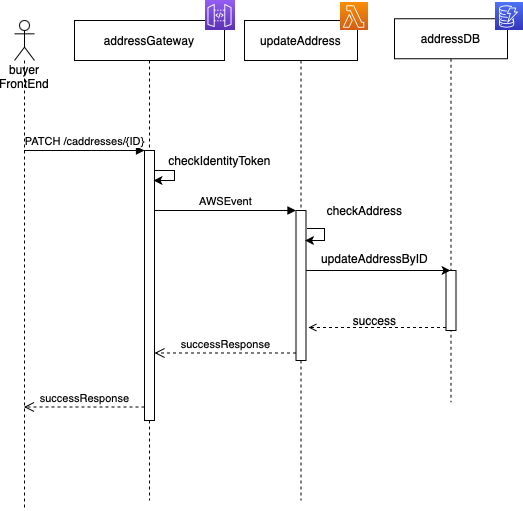
\includegraphics[scale=0.5]{Immagini/Backend/ModificaIndirizzo.png}
	\caption{Modifica di un indirizzo di spedizione}
	\label{fig:DiagrammaModificaindirizzo}
\end{figure}
All'interno della piattaforma l'acquirente può aggiungere, eliminare o modificare gli indirizzi di spedizione inseriti, il diagramma rappresenta la collaborazione delle tecnologie per effettuare quest'ultima operazione.
\subsubsection{Pagamento e creazione di un ordine}
\begin{figure}[H]
	\centering
	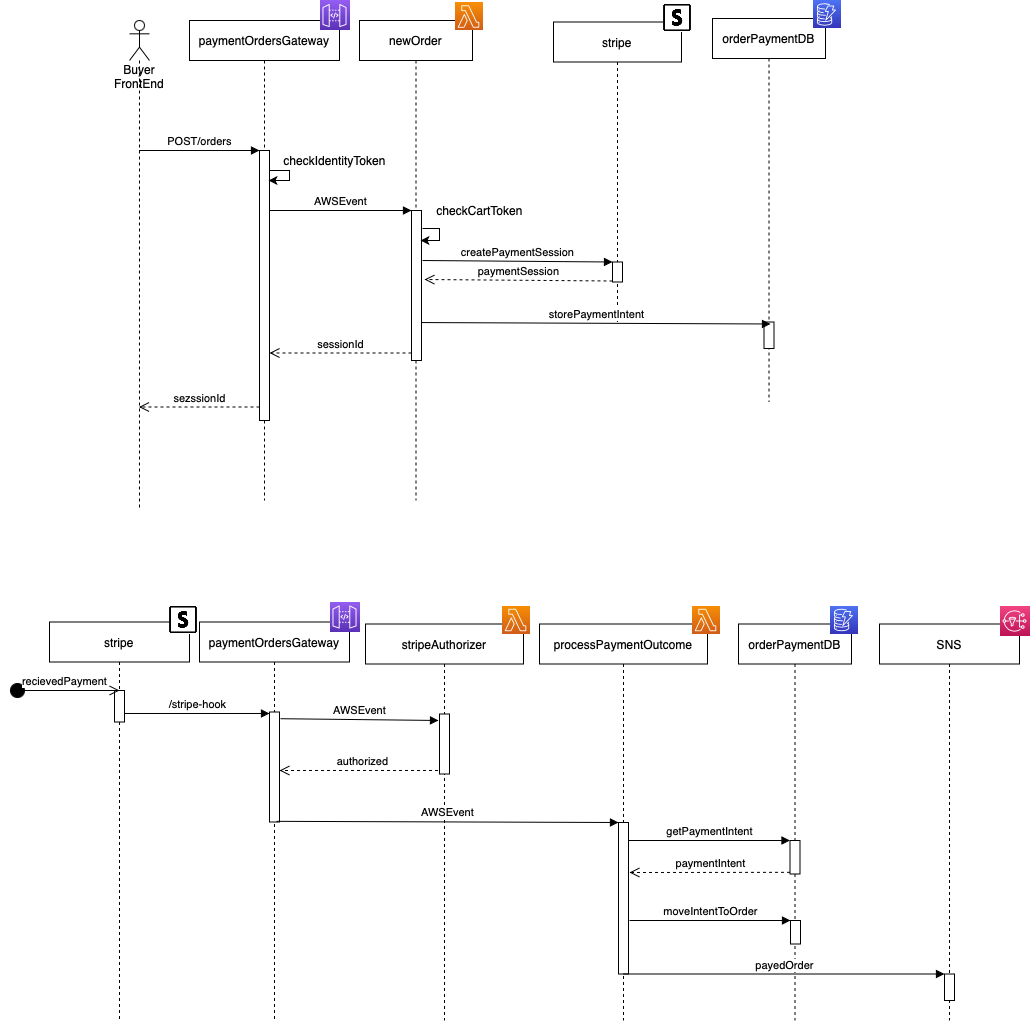
\includegraphics[scale=0.5]{Immagini/Backend/Diagrammiseq.png}
	\caption{Nuovo ordine e pagamento dello stesso}
	\label{fig:Diagrammiseq}
\end{figure}
I precedenti diagrammi rappresentano le tecnologie che entrano in gioco quando l'acquirente della piattaforma effettua un pagamento e, se questo è andato a buon fine, di conseguenza quanto inserito all'interno del carrello verrà trasformato in un'ordine effettuato e di conseguenza visualizzabile dall'utente all'interno dell'elenco degli ordini effettuati.
\newpage
\section{Frontend}\label{Frontend}
\subsection{Descrizione generale}
\begin{figure}[H]
	\centering
	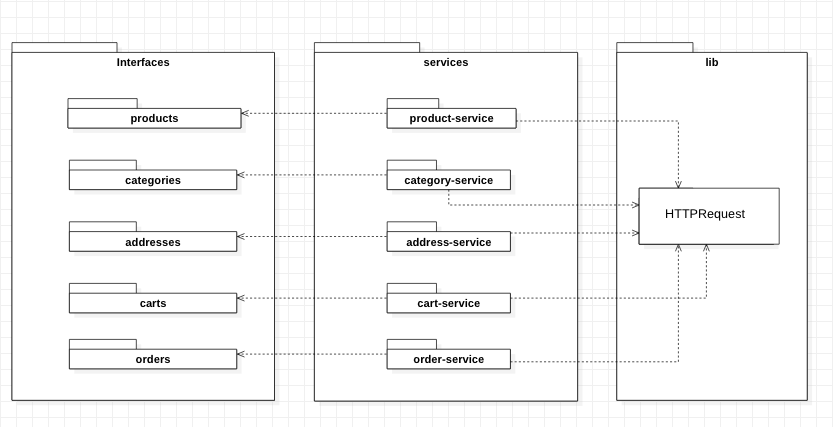
\includegraphics[scale=0.6]{Immagini/Frontend/DiagrammadeiPackage.png}
	\caption{Diagramma dei package}
	\label{fig:fe-packages}
\end{figure}
Il diagramma rappresenta le dipendenze tra le classi che individuano i \glo{microservizi}.
Il package \textbf{interfaces} contiene tutti i tipi che verranno utilizzati dal frontend.
La classe \textbf{HTTPRequest} è stata implementata per centralizzare le chiamate \glo{HTTP} e permettere il controllo dei tipi, consiste in un wrapper della libreria nativa fetch andando a ridefinire i metodi GET, POST, PATCH, PUT e DELETE. Ottiene la variabile d'ambiente contenente l'url del server dal file di configurazione relativo di dotenv, dal costruttore gli verrà passato l'url alla specifica \glo{API} il quale verrà aggiunto all'url precedente e su questo sarà possibile invocare i metodi precedentemente dichiarati.
Il package \textbf{services} rappresenta l'unico punto di collegamento tra i microservizi del backend e il frontend, tramite \glo{API} redatte utilizzando SwaggerHub, i vari servizi al suo interno andranno a invocare HTTPRequest per comunicare con il backend attraverso i metodi definiti.
I microservizi individuati e utilizzati per il frontend sono:
\begin{itemize}
	\item \textbf{Product;}
	\item \textbf{Address;}
	\item \textbf{Categories;}
	\item \textbf{Orders;}
	\item \textbf{Carts.}
\end{itemize}
\subsubsection{Esempio di funzionamento}
Di seguito si riporta il diagramma delle classi relativo al funzionamento del microservizio \textbf{product}. Come si può vedere è presente un'interfaccia ProductService che viene implementata dalla classe ProductServiceFetch e ogni suo metodo istanzia un oggetto HTTPRequest per l'API di interesse. È possibile implementare l'interfaccia ProductService diversamente rispetto a quanto rappresentato senza la necessità di modificare il codice utilizzatore, attraverso la modifica della variabile d'ambiente NEXT\_PUBLIC\_SERVICE\_METHOD sarà possibile scegliere quale implementazione utilizzare altrimenti verrà di default selezionata l'implementazione ProductServiceFetch. 
Per poter procedere con lo sviluppo della parte dei prodotti del frontend parallelamente con il backend, lo sviluppatore ha a disposizione la classe ProductServiceMock la quale ritornerà i dati predefiniti senza dover richiamare il server, basterà impostare la variabile NEXT\_PUBLIC\_SERVICE\_METHOD="mock".
\begin{figure}[H]
	\centering
	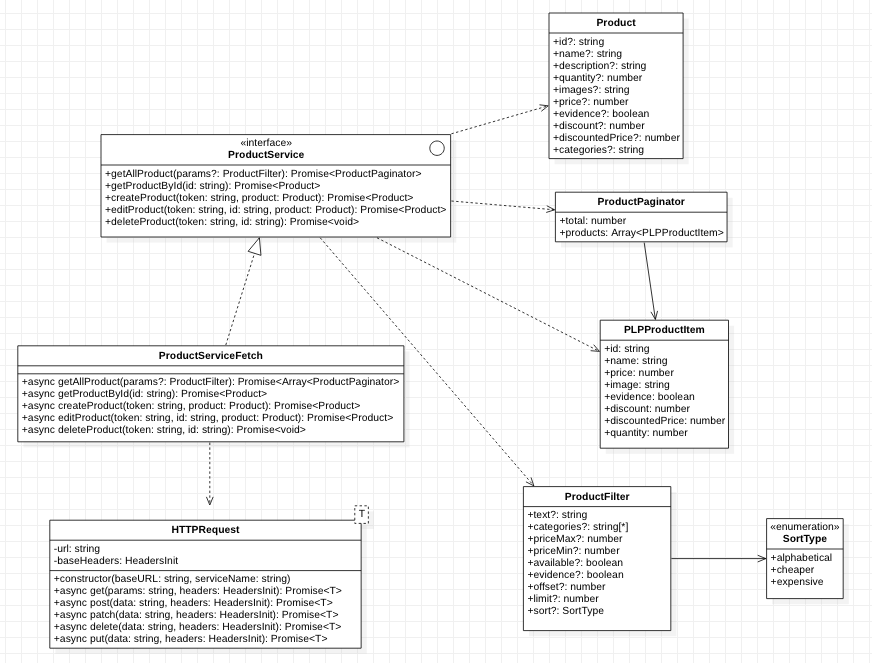
\includegraphics[width=\textwidth]{Immagini/Frontend/ProductService.png}
	\caption{Microservizio Product}
	\label{fig:fe-productservice}
\end{figure}


\end{document}